\documentclass{beamer}
\usepackage[utf8]{inputenc}
\usepackage[ngerman]{babel}
\usepackage{beamerthemeshadow}
\usepackage{calc}
\usepackage{ifthen}
\usepackage{multimedia}
\usepackage{listings}

\usepackage{pgf-pie}

\lstset{
	basicstyle=\ttfamily\scriptsize,
	language=bash,
	showspaces=false,
	showstringspaces=false,
	showtabs=false,
}

\usepackage{tikz}
\usetikzlibrary{shapes.geometric, arrows}
\usetikzlibrary{calc}
\usetikzlibrary{positioning}

\tikzstyle{component} = [rectangle, rounded corners, minimum width=1cm, minimum height=1cm,text centered, draw=black, fill=red!30]
\tikzstyle{power} = [rectangle, rounded corners, minimum width=1cm, minimum height=1cm,text centered, draw=black, fill=red!30]
\tikzstyle{driver} = [rectangle, rounded corners, minimum width=1cm, minimum height=1cm,text centered, draw=black, fill=green!30]
\tikzstyle{logic} = [rectangle, rounded corners, minimum width=1cm, minimum height=1cm,text centered, draw=black, fill=blue!30]
\tikzstyle{flowchart-block} = [rectangle, rounded corners, minimum width=1.75cm, minimum height=1.75cm,text centered, text width=1.5cm, draw=black, fill=blue!30]
\tikzstyle{flowchart-decision} = [diamond, rounded corners, minimum width=1.75cm, minimum height=1.75cm,text centered, text width=1.5cm, draw=black, fill=green!30]

\usepackage{caption}
\usepackage{bchart}
\usepackage{wrapfig}
\usepackage{ulem}

\newcommand{\group}{Team 39 -- accefa}


\title{Autonome Ballwurfmaschine}
\subtitle{Produktentwicklung 1}
\institute{Hochschule Luzern\\Technik \& Architektur}
\author{\group}

\begin{document}
	% contents
\renewcommand{\abstractname}{Abstract}
\begin{abstract}
Die Erstellung eines Lösungskonzeptes verlangt nach einer gründlichen
Recherche für sämtliche Kernelemente und Produktkriterien der gegebenen
Problemstellung. Dies betrifft insbesondere die technischen und 
funktionalen Aspekte. 

Für die vollständige Erfassung der Problembereiche ist eine kreative 
und heuristische Methode zu Anwendung gekommen, welche auch als 
morphologischer Kasten bekannt ist. Diese hat sowohl den Aufbau
als auch den Inhalt dieser Technologierecherche geprägt.

Die vorliegende Recherche umfasst sämtliche Fachbereiche der 
Problemstellung und unterscheidet diese auch nicht weiter um die
konkrete Lösungsfindung nicht zu beeinflussen. Für die
flexible Anwendung der Ergebnisse ist eine Tabelle erstellt worden,
welche alle relevanten Daten und Quellen direkt verlinkt.
\end{abstract}

\newpage
\tableofcontents
\newpage
\section{Funktionen des Systems}
Um die benötigten Funktionen unseres System zu eruieren, wird der Ablauf des gesamten Systems bildlich dargestellt. Der Ablauf startet bereits mit einem Startsignal und endet mit dem Stoppsignal.

\begin{figure}[h!]
\centering
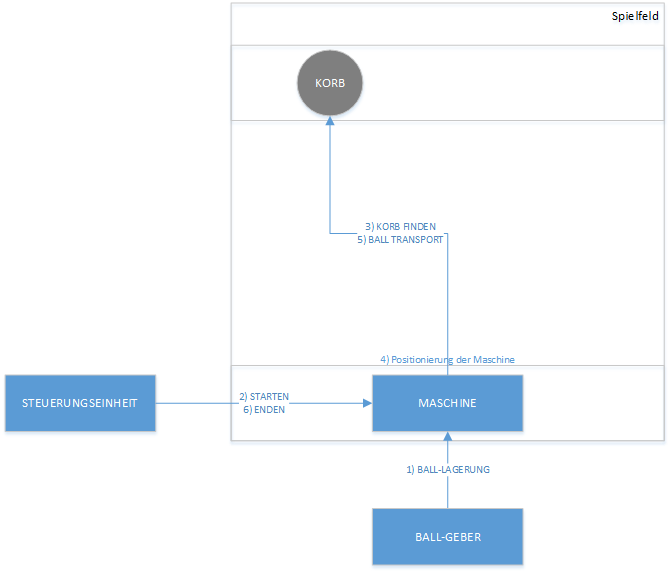
\includegraphics[width=0.7\linewidth]{../../fig/ablauf-transport}
\caption[Gesamter Ablauf des Transports]{Gesamter Ablauf des Transports}
\label{fig:ablauf-transport}
\end{figure}

Auf der Abbildung \ref{fig:ablauf-transport} sind die einzelnen Schritte zu erkennen, welche durchlaufen werden müssen. Die Nummerierung stellt die Reihenfolge dar. Die STEUERUNGSEINHEIT ist eine externe Einheit, welche mit der MASCHINE kommuniziert. Die MASCHINE ist dann für den eigentlichen Transport der Bälle verantwortlich. Die Aktion des BALL-GEBER kann eine manuelle Interaktion mit der MASCHINE sein.\\
\\
Im ersten Schritt übergibt der BALL-GEBER die Bälle der Maschine, darauf folgt ein Startsignal der STEUERUNGSEINHEIT. Anschliessend muss die MASCHINE den Korb im Spielfeld orten und sich im Schritt 4 entsprechend positionieren. Nach dem Transport der Bälle sendet die MASCHINE ein Stopsignal an die STEUERUNGSEINHEIT.

\subsection{Funktionen}
Aus diesen Aktivitäten lassen sich die Funktionen ableiten, welche das System leisten muss.\\
 
\begin{description}
    \item [Ball-Lagerung] Der Ball-Geber übergibt im Schritt 1 der 
        Maschine die Bälle. Die Bälle müssen danach von der Maschine 
        gelagert werden.
    \item [Kommunikation] Die Steuerungseinheit und die Maschine müssen 
        in den Schritten 2 und 6 miteinander kommunizieren.
    \item [Ortung des Korbs] Im Schritt 3 muss der Korb geortet werden.
    \item [Maschinen Positionierung] Im Schritt 4 kann die ganze Maschine
    positioniert werden. Möglicherweise fährt es irgendwo hin.
    \item [Maschinen Ausrichtung] Im Schritt 4 kann sich die Maschine alternativ
    auch ausrichten. Damit ist gemeint, dass auf der Maschine eventuell
    eine bewegliche Achse installiert ist.
    \item [Transport der Bälle] Im vorletzten Schritt werden die Bälle 
        in den Korb transportiert.
    \item [Energieversorgung] Dieser Punkt lässt sich nicht direkt aus 
        dem Ablauf erkennen. Jedoch ist diese Funktion zentral, denn 
        die Steuerungseinheit und auch die Maschine müssen mit Energie 
        versorgt werden. Daher wird dieser Punkt explizit aufgenommen.
    \item [Computer] Auch dieser Punkt ist sehr wichtig und nicht direkt 
        ableitbar aus dem Ablauf. Die Maschine und auch die 
        Steuerungseinheit müssen möglicherweise Berechnung vornehmen.
\end{description}

\newpage
\section{Funktionsübersicht}
In dieser Übersicht werden alle erarbeiteten Funktionen aufgelistet. Dazu werden konkrete Umsetzungsmöglichkeiten genannt, welche die Funktion umsetzen bzw. unterstützen könnten.\\
\\

\begin{table}[h!]
	\centering
	\begin{tabular}{l p{3cm} p{4.5cm} p{8cm}}
		Nr & Funktion & Ideen & Beschreibung \\
		\hline
		
		1 & Energieversorgung & A Elektrisch (Netz) & Elektrizität mit dem Stromnetz als Quelle. \\
		 &  & B Elektrisch (Akku) & Elektrizität mit einem Akku als Quelle. \\
		 &  & C Pneumatisch (direkt) &  Luftdruck mit dem Druckluftnetz als Quelle. \\
		 &  & D Pneumatisch (Drucktank) & Luftruck mit einem Drucktank als Quelle. \\
		 &  & E Dampf & Dampf als Energiequelle. \\
		
	
	    2 & Ball-Lagerung & A Magazin & Ein Magazin als Lagerung. \\
	    &  & B Korb & Ein Korb als Lagerung. \\
	    &  & C Netz & Ein Netz als Lagerung. \\
	    &  & D Rohr & Ein Rohr als Lagerung. \\
	    
	   
	    
	    3 & Kommunikation & A Handy & Ein Handy als externer Kommunikationspartner. \\
	    &  & B Laptop & Ein Laptop als externer Kommunikationspartner. \\
	    &  & C Fernbedienung & Eine Fernbedienung als externer Kommunikationspartner. \\
	    &  & D Akustisches Signal & Datenübertragung per Akustik. \\
	    &  & E Lichtsignal & Datenübertragung per Licht. \\
	    
	   
	    
	    4 & Ortung des Korbs & A Ultraschall & Mittels Ultraschall den Ort des Korbs detektieren. \\
	    &  & B Laser & Mittels Laser den Ort des Korbs detektieren. \\
	    &  & C Optik & Mittels Optik den Ort des Korbs detektieren (Kamera). \\
	    &  & D Wärmebild & Mittels Wärmebild den Ort des Korbs detektieren. \\
	    &  & E Radar & Mittels Radar den Ort des Korbs detektieren. \\
		
	
		
	    5 & Maschinen Positionierung & A fix & Maschine fixiert an einem Ort. \\
		 &  & B Spring in Korb & Maschine springt komplett in den Korb. \\
		 &  & C Fährt & Maschine fährt an einen Ort um sich zu positionieren. \\
		 &  & D Rollt & Maschine rollt an einen Ort um sich zu positionieren. \\
		 &  & E Fliegt & Maschine fliegt. \\
		
	
	    6 & Transport der Bälle & A Drehräder (Reibung) & Die Bälle werden durch die Reibung an den Drehräder beschleunigt. \\
	     &  & B Drehräder (Formschlüssig) & Die Bälle gewinnen an Geschwindigkeit durch die formschüssigen Elemente an den Drehrädern.  \\
	     &  & C Katapult & Die Bälle werden katapultiert. \\
	     &  & D Ausfahrbarer Zylinder & Ein Zylinder, welcher einen Stossimpuls gibt.  \\
	     &  & E Fallbeschleunigung & Die Bälle fliegen aus der Höhe in die Tiefe. \\
	     &  & F Feder & Mit Federkraft die Bälle Beschleunigung.  \\
	     &  & G Luft & Die Bälle mit Luft (dran blasen) beschleunigen.  \\
		 
		7 & Computer & A Bordcomputer & Steuereinheit der Maschine. \\
		
	
		
		 8 & Maschinen Ausrichtung & A Vertikale Ausrichtung & Maschine richtet sich selbst vertikal aus. \\
		 &  & B Horizontale Ausrichtung & Maschine richtet sich horizontal aus. \\
		 
	\end{tabular}
	\caption{Funktionsübersicht}
	\label{tab:quelle}
\end{table}

\newpage
\section{Quellen}

%\begin{table}
	\begin{zebralongtable}{c l c l}
		\centering
		\textbf{Referenz} & \textbf{Bezeichnung} & \textbf{Bewertung} & \textbf{Quelle} \\
		\hline
        	1A 
			& Stecker-Netzteil 
			& 3 
			& \href{http://www.conrad.ch/ce/de/product/514218/Stecker-Netzteil-Festspannung-VOLTCRAFT-FPPS-9-36W-9-VDC-400-mA?ref=searchDetail}{Conrad} \\
        	1A 
			& DIY Trafonetzteil 
			& 2 
			& \href{http://de.wikipedia.org/wiki/Netzteil#Trafonetzteil}{Wikipedia} \\
        	1A 	
			& DIY Schaltnetzteil 
			& 2 
			& \href{http://de.wikipedia.org/wiki/Netzteil#Schaltnetzteil}{Wikipedia} \\
        	1A 	
			& Fachbuch Schaltnetzteile 
			& 2 
			& \href{http://www.buchhaus.ch/start/detail/ISBN-9783834816467/Schlienz-Ulrich/Schaltnetzteile-und-ihre-Peripherie}{Buchhaus} \\
        	1A 
			& Labornetzteil 
			& 1 
			& \href{http://ch.farnell.com/tenma/72-10480/labornetzteil-1fach-30v-3a/dp/2251946}{Farnell} \\
        	1B 
			& Powerbank 
			& 4 	
			& \href{http://www.conrad.ch/ce/de/product/776952/iGo-Powerbank-1-USB-4700-mAh-schwarz-LiPo-4700-mAh-PS00319-0002-Powerbank-1-USB-Mobile-Stromversorgung-Zusatzakku-En?ref=searchDetail}{Conrad} \\
        	1B 	
			& DIY LiPo Supply 
			& 3 
			& \href{http://www.elv.ch/li-ion-lipo-ladegeraet-lipo-4-komplettbausatz.html}{ELV} \\
        	4A 
			& Ultraschallmodul 
			& 3 
			& \href{http://www.parallax.com/product/28015}{Parallax} \\
        	4A 
			& Ultraschallmodul 
			& 3 
			& \href{https://github.com/luxeria/e-wall}{LuXeria} \\
        	4B 
			& Lasermodul 
			& 1 
			& \href{http://www.parallax.com/product/28044}{Parallax} \\ 
		4C	
			& Intelligentes Kameramodul
			& 3
		& \href{https://www.kickstarter.com/projects/254449872/pixy-cmucam5-a-fast-easy-to-use-vision-sensor}{Pixy} \\
		% Alex Sutes Part        
		3A/3B 
			& Einführung in die Bluetooth Technologie mittels Java 
			& 2 
			& \href{https://today.java.net/pub/a/today/2004/07/27/bluetooth.html}{java.net} \\
        	3B 
			& Bluetooth Datentransfer von der Android Plattform aus 
			& 2 
			& \href{http://tsicilian.wordpress.com/2012/11/06/bluetooth-data-transfer-with-android/}{tsicilian.wordpress.com} \\
        	3A/3B 
			& Übersicht Kabellose Datenübertragung 
			& 2 
			& \href{http://de.wikipedia.org/w/index.php?title=Kabellose_\%C3\%9Cbertragungsverfahren&redirect=no}{Wikipedia} \\
        	3E 
			& Optischer Richtfunk 
			& 1 
			& \href{http://de.wikipedia.org/wiki/Optischer_Richtfunk}{Wikipedia} \\
        	4E 	
			& Radar-Sensoren 
			& 1 
			& \href{http://www.conrad.ch/ce/de/overview/0231510/Radar-Sensoren}{Conrad} \\
        	4D 	
			& Wärmebildkameras 
			& 1 
			& \href{http://de.wikipedia.org/wiki/W\%C3\%A4rmebildkamera}{Wikipedia} \\
        	4D 
			& Konkretes Wärmebild Kamera Produkt 
			& 1 
			& \href{http://www.mobilefun.co.uk/flir-one-personal-thermal-imaging-case-for-iphone-5-5s-p43472.htm}{Flire-One} \\
        	7A 
			& Raspberry PI - Gängiger Minicomputer 
			& 1 
			& \href{http://de.wikipedia.org/wiki/Raspberry_Pi}{Wikipedia} \\
        	7A 
			& Raspberry PI - Bluetooth Adapter 
			& 3 
			& \href{http://www.rasppishop.de/raspberry-pi-welt/netzwerk/w-lan/149/bluetooth-dongle-v2.0-adapter-fuer-raspberry-pi}{rasppishop.de} \\
        	7A 
			& Raspberry PI - Bluetooth Adapter 2 
			& 3 
			& \href{http://elinux.org/RPi_USB_Bluetooth_adapters}{elinux.org} \\
        	7A 
			& Raspberry PI - Infrared 
			& 2 
			& \href{https://learn.adafruit.com/using-an-ir-remote-with-a-raspberry-pi-media-center/overview}{adafruit.com} \\
        	7A 
			& Alternativen zum Raspberry PI 
			& 2 
			& \href{http://www.netznews.eu/10-raspberry-pi-alternativen-im-kurzportraet/}{netznews.eu} \\
        	4C 
			& Bilderkennungsverfahren 
			& 2 
			& \href{http://en.wikipedia.org/wiki/Outline_of_object_recognition}{Wikipedia} \\
        	4C 
			& Image Processing 
			& 2 
			& \href{http://en.wikipedia.org/wiki/Image_processing}{Wikipedia} \\
        	4C 
			& Image Processing - Principles and Applications 
			& 2 
			& \href{http://books.google.co.in/books?id=smBw4-xvfrIC&lpg=PP1&dq=image\%20processing\%20ajoy\%20ray&pg=PP1#v=onepage&q=&f=false}{Buch} \\
        	4C 
			& Image Processing - Einführung in Java 
			& 2 
			& \href{ http://imagingbook.com/}{Buch} \\
        	4C 
			& Bilderkennung mittels Java 
			& 2 
			& \href{https://www.medien.ifi.lmu.de/lehre/ss07/mt/mtB3b.pdf}{medien.ifi.lmu.de} \\
        	4D 
			& Audio Processing Übersicht 
			& 1 
			& \href{http://en.wikipedia.org/wiki/Audio_signal_processing}{Wikipedia} \\
        	4D 
			& Audio Processing Java Library 
			& 1 
			& \href{http://www.beadsproject.net/}{beadsproject.net} \\
        	3C 
			& Programmierbare Fernbedienungen 
			& 1 
			& \href{http://lifehacker.com/5901930/five-best-universal-remote-controls}{lifehacker.com} \\
		% Christian Schürchs part
         	F6 
			& Feder 
			& 2 
			& \href{http://de.wikipedia.org/wiki/Feder_(Technik)}{Wikipedia} \\
		C6 
			& Katapult 
			& 2 
			& \href{http://de.wikipedia.org/wiki/Katapult}{Wikipedia} \\
		C6 
			& Balliste 
			& 2 
			& \href{http://de.wikipedia.org/wiki/Balliste}{Wikipedia} \\
		C6 
			& Armbrust 
			& 2 
			& \href{http://de.wikipedia.org/wiki/Armbrust}{Wikipedia} \\
		C6 
			& Schleuder 
			& 2 
			& \href{http://de.wikipedia.org/wiki/Zwille}{Wikipedia} \\
		A6 
			& Räder 
			& 2 
			& \href{http://www.fta.ch/de/r/raeder-2000.html}{FTA} \\
		D6 
			& Elektrozylinder 
			& 3 
			& \href{http://www.parkem.ch/medien/produkte/bewegungsmechanik/pdf/mechanik_et_tech_de_190-550011.pdf}{Parkem} \\
        	D6 
			& Elektrozylinder 
			& 3 
			& \href{http://www.festo.com/net/de_de/SupportPortal/Details/219992/PressArticle.aspx}{Festo} \\
        	n.a. 
			& Pitching Machine 
			& 2 
			& \href{http://en.wikipedia.org/wiki/Pitching_machine}{Wikipedia} \\
        	n.a.
			& Toss Machine 
			& 2 
			& \href{https://www.google.ch/search?q=toss+machine&ie=utf-8&oe=utf-8&aq=t&rls=org.mozilla:de:official&client=firefox-a&channel=sb&gfe_rd=cr&ei=zk4uVPT4Mseh7AbexYGAAg}{Google} \\
		n.a. 	& Projectiles 
			& 2 
			& \href{http://physics.info/projectiles/}{Physics} \\
		% Christian Spychers part
        	6A 
			& Video Abwurfmechanismus 
			& 3 
			& \href{http://www.youtube.com/watch?v=ehrB93rbLoM}{youtube.com} \\
         	6A 
			& Video Abwurfmechanismus 
			& 2 
			& \href{http://www.youtube.com/watch?v=Za3fQ1TSFrY}{youtube.com} \\
		6A 
			& Video Abwurfmechanismus 
			& 2 
			& \href{http://www.youtube.com/watch?v=MSjCmDsDnNU}{youtube.com} \\
          	6A 
			& Video Abwurfmechanismus 
			& 2 
			& \href{http://www.youtube.com/watch?v=oZjx7F1doGs}{youtube.com} \\
		1D / 6D 
			& Pneumatik Komponenten und Drucklufttechnik 
			& 2 
			& \href{http://www.festo.com/net/startpage/}{Festo} \\
		6G 
			& Elektroventile für Abschuss Pneumatisch 
			& 3 
			& \href{http://www.distrelec.ch/Web/Downloads/a_/de/VDW-A_cat_EUS70-49A_de.pdf?mime=application%2Fpdf}{distrelec.ch} \\
          	
		6G 
			& Elektroventile für Abschuss Pneumatisch 
			& 3 
			& \href{http://www.festo.com/cat/de-ch_ch/products_MHJ}{festo.com} \\
		% Adriano Valsangiacomo part 
		5A 
			& Gummifüsse 
			& 1 
			& \href{http://www.conrad.de/ce/de/Search.html?search=Gummif%C3%BCsse&initial=true}{Conrad} \\
		5C 
			& Raeder 
			& 1 
			& \href{http://www.haertle.de/RC+Modellbau/RC+Car+Zubehoer/Reifen+Felgen+Raeder/}{Haertle} \\
		5C 
			& RC-Elektromotoren 
			& 2 
			& \href{http://www.conrad.ch/ce/de/overview/1202032/Auto-Truckmodell-Elektromotore}{Conrad} \\
		5C 
			& Lego lösung 
			& 1 
			& \href{http://www.coolbricks.com/motoren}{CoolBricks} \\
		5E 
			& Motor für Quadrocopter 
			& 1 
			& \href{http://www.goodluckbuy.com/xxd-a2212-1000kv-brushless-motor-for-quadcopter-multicopter-4-pack.html}{GoodLuckBuy} \\
		5E 
			& Motor speed controller für Quadcopter 
			& 1 
			& \href{http://www.goodluckbuy.com/30a-brushless-motor-speed-controller-programable-esc-2a-bec-for-quadcopter-4-pack.html}{GoodLuckBuy} \\
		5E 
			& Steuerung von Quadrocopter 
			& 2 
			& \href{http://www.rc-drohnen.de/antrieb-und-steuerung-von-quadrocopter/}{RC-Drohnen} \\
		6E 
			& Schwerefeld 
			& 1 
			& \href{http://de.wikipedia.org/wiki/Schwerefeld}{Wikipedia} \\
		2A
			& Bau-Normröhren (Kunststoff)
			& 1
			& \href{https://www.hornbach.ch/shop/suche/articles-overview-de.html?wt.tsrc=&blistsize=&wt.srch=&wt.mc_id=&bfilter=&bdvra=&bsearch=rohr&cid=193922}{Hornbach} \\
		2B
			& Trichter
			& 1
			& \href{https://www.hornbach.ch/shop/suche/articles-overview-de.html?wt.tsrc=&blistsize=&wt.srch=&wt.mc_id=&bfilter=&bdvra=&bsearch=trichter&cid=193983}{Hornbach} \\
		2C
			& Netz
			& 1
			& \href{https://www.hornbach.ch/shop/suche/articles-overview-de.html?wt.tsrc=&blistsize=&wt.srch=&wt.mc_id=&bfilter=&bdvra=&bsearch=netz&cid=194061}{Hornbach} \\
		2D
			& Bau-Normröhren (Kunststoff)
			& 1
			& \href{https://www.hornbach.ch/shop/suche/articles-overview-de.html?wt.tsrc=&blistsize=&wt.srch=&wt.mc_id=&bfilter=&bdvra=&bsearch=rohr&cid=193922}{Hornbach} \\
		5B
			& Springender Roboter (Boston Dynamics)
			& 1
			& \href{https://www.youtube.com/watch?v=6b4ZZQkcNEo}{YouTube} \\
		8A
			& Winkelsensor
			& 1
			& \href{http://www.asm-sensor.com/de/winkelsensor/winkelsensor.html}{ASM} \\
		8B
			& Servomotoren
			& 1
			& \href{http://www.conrad.ch/ce/de/Search.html;jsessionid=6156D4736D5FAA96C7114575FB47C742.ASTPCEN27?search=servomotor&searchType=mainSearchBar}{Conrad} \\
		\caption{Quellen zur Technologierecherche}
	\end{zebralongtable}
%\end{longtable}

\newpage
\section{Patente}

\begin{table}[h!]
	\centering
	\begin{tabular}{l l l l l}
		Nr. & Patentnummer & Pub. Datum & Titel & Patentanmelder \\
		\hline
        
        1 & \href{http://www.google.com/patents/US6202636}{US6202636} & 20.03.2001 & Pitching machine & The Lobit Partnership  \\
        
        
        
	\end{tabular}
	\caption{Patente-tabelle}
	\label{tab:quelle}
\end{table}


\end{document}
